\section{Rekonstruktion}\label{sec:implementation-reconstruction}

In diesem Abschnitt werden die einzeln Schritte zum Rekonstruieren der Korrespondenzen erklärt, die im vorherigen Prozess gebildet worden sind. 
Für die Rekonstruktion wird die Klasse \emph{SceneReconstructor} in der Datei \emph{reconstruction.hpp} definiert und in \emph{reconstruction.cpp} implementiert (siehe XXX und XXX). 
Die Klasse besitzt einen Konstruktor, welche eine Instanz der Calibration Klasse als Argument benötigt. 
Mit der Instanz wird die private Member-Variable \emph{calbiration} instanziiert, so dass sie später zum Berechnen der Projektionsmatrix verwendet werden kann.
Des Weiteren wird die öffentliche Methode \emph{reconstructScenes} definiert.
Mit dem Iterator werden in der Methode die korrespondierenden Bildpunkte rekonstruiert.
Dabei wird darauf geachtet, dass die rekonstruierten Punkte der einzelnen Paare später auch zusammen passen.
Wie in XXX zusehen ist, werden einige weitere private Methoden für die Klasse definiert.
Diese Implementieren bestimmte Berechnungen für die Rekonstruktion, die in den folgenden Paragrahen näher erläutert werden.
Für jedes Bildpaar wird die Rekonstruktion in den folgenden 5 Schritten durchgeführt:

\begin{enumerate}
    \item Lokale Rotation \& Translation bestimmen
    \item globale Translation berechnen
    \item Projektionsmatrix berechnen
    \item Triangulation
    \item Skalieren
        \begin{enumerate}
            \item skalierte, globale Translation berechnen
            \item Projektionsmatrix berechnen
            \item Triangulation
        \end{enumerate}
\end{enumerate}

Im ersten Schritt wird für das aktuelle Bildpaar die Rotation und Translation der rechten Kamera im Bezug auf die Linke bestimmt.
Wie in \cref{sec:essential-mat} beschrieben, wird dazu die essentielle Matrix berechnet und in $R$ und $t$ zerlegt.
OpenCV bietet dafür die Funktionen \emph{findFundamentalMat}~\cite{opencv_doc_essential_matrix} und \emph{recoverPose}~\cite{opencv_doc_recover_pose} an.
In Zeile XXX des Listings XXX wird findFundamentalMat aufgerufen. 
Hierbei werden die korrespondierenden Bildpunkte der beiden Bilder und die Kalibrierungsmatrix übergeben.
Mit den weiteren drei Argumenten wird der angewendete Algorithmus gewählt und angepasst.
Es kann zwischen \emph{RANSAC} (random sampling with consensus) und \emph{LMeDS} (least median of squares) gewählt werden.
Hier wird der RANSAC Algorithmus gewählt, da laut~\cite[Kapitel 18, 664]{kaehler_2016} RANSAC resistenter gegen Ausreißer und Rauschen im Bild ist als LMeDS. % TODO: ggf noch ein Satz zu warum das gut ist, also dass wir Ausreißer in den Matches und evt. schlete Bilder erwarten
Laut der OpenCV Dokumentation~\cite{opencv_doc_essential_matrix}, muss bei RANSAC ein Threshold in Pixel angegeben werden, mit dem die Ausreißer bestimmt werden.
Dieser wird bei bei dem niedrigsten möglichen Wert, hier 1 Pixel, belassen.
Genauere Details zu den beiden Algorithmen sind nötig werden hier nicht näher erklärt.
Bei Interesse können die originalen Arbeiten zu RANSAC (siehe~\cite{fischler_81}) und LMeDS (siehe~\cite{inui_03}) gelesen werden.
Mit dem letzten Argument der Methode, wird in einem Vektor vermerkt, welche der Matches Ausreißer sind.
Dieser Vektor wird in einem späteren Schritt genutzt, um die rekonstruierten Punkte zu filtern.
Die somit bestimmte essentielle Matrix wird dann in XXX mit recoverPose in die Rotationsmatrix $R$ und den Translationsvektor $t$ zerlegt.
% Dazu werden neben der essentiellen Matrix auch die wieder die korrespondierenden Bildpunkte und die Kalibrierungsmatrix angegeben.
% erkläre kurz die Methode

Mit $R$ und $t$ ist es bereits möglich die korrespondierenden Bildpunkte zu rekonstruieren.
Jedoch werden diese in einem Koordinatensystem ausgedrückt, dass durch die linke Kamera definiert ist, wodurch die Punkte aller Bildpaare nicht zusammengeführt werden können.
Daher wird im dritten Schritt die \emph{globale Transformation} $T_n$ berechnet, die die Rotationen und Translationen der vorherigen Bildpaare berücksichtigt.
Somit bezieht sich die Position der rechten Kamera des nten Bildpaars auf die linke Kamera des ersten Bildpaars 
Es gilt:
\[ T_n = T_{n-1} \cdot \begin{bmatrix}
            R & t \\
            0 & 1 \\
        \end{bmatrix}
    \] 
Dabei ist $T_0$ die $4 \times 4$ Identitätsmatrix.
Die Berechnung ist in XXX in Zeile XXX implementiert.
$T_{n-1}$ wird von der Methode \emph{getPreviousTransform} der ImagePair Klasse als Argument übergeben. % TODO: ggf. getPreviousTransform erklären, wenn nicht bereits getan
Zusätzlich wird in XXX die Hilfsmethode \emph{combineToTranformation} implementiert, die eine $3\times3$ Rotationsmatrix und einen Translationsvektor zu einer $4\times4$ Transformationsmatrix zusammensetzt.

In der getPreviousTransform wird auch der vierte Schritt ausgeführt, in dem die Projektionsmatrix berechnet wird.  
Dazu ist es nötig $T_n$ in die Rotationsmatrix $R_n$ und den Translationsvektor $t_n$ aufzuteilen. 
% $R_n$ und $t_n$ sind hierbei die Rotation und Translation der rechten Kamera des nten Bildpaares im Bezug auf die linke Kamera des ersten Paars.
Es gilt $T_n = \begin{bmatrix}
                R_n & t_n \\
                0 & 1 \\
            \end{bmatrix}$
Die Aufteilung wird ist in der Methode \emph{getFromTransformation} in XXX implementiert.
Anschließend wird die Projektionsmatrix $P$ mit $P = K[R|t]$ berechnet, und wird in der Methode \emph{getProjection} in XXX implementiert.

In Schritt 4 werden die Bildpunkte mit der Methode \emph{triangulatePoints} von Opencv rekonstruiert.
Sie benötigt als Argumente die Projektionsmatrizen beider Kameras, sowie die Korrespondenzen aus beiden Bilder.
Die Projektionsmatrix der linken Kamera entspricht der Projektionsmatrix des vorherigen Bildpaars. 
Auf sie kann durch die Methode \emph{getPreviousProjection} der ImagePair Klasse zugegriffen werden.% gff. Methode erklären falls es noch nicht getan worden ist
Die rekonstruierten Punkte werden von triangulatePoints als eine $4\times N$ Opencv Matrix zurückgegeben.
Dabei entspricht eine Spalte der Matrix einen einzeln Punkt im Raum in homogenen Koordinaten.

Die Rekonstruktion des ersten Bildpaares ist mit diesem Schritt bereits vollendet.
Durch die Methode \emph{setReconstruction} der ImagePair Klasse werden die Ergebnisse der Rekonstruktion für die aktuelle ImagePair Instanz gespeichert.
Dieser Methode werden die Projektionsmatrix, die Transformationsmatrix, die rekonstruierten Punkte und die Maske der Ausreißer als Argumente übergeben. 
Wie in XXX zusehen ist, werden die Projektions- und Transformationsmatrix einfach den Member-Variablen zugewiesen.
Die rekonstruierten Punkte werden dahingegen gefiltert und zu einem vector<cv::Point3f> konvertiert.
Dabei werden alle Ausreißer, die durch die Maske angegeben werden, sowie alle Punkte mit einem negativen Z-Wert gefiltert.
Grund dafür ist, dass die Richtung der Kameras in Richtung der Z-Achse definiert ist.
Ein Punkt mit negativer Z-Achse liegt also hinter der Kamera, was physikalisch unmöglich ist und daher gefiltert werden muss.
Die Punkte liegen in homogenen Koordinaten vor, weswegen jeder Punkt vor dem Filtern durch das vierte Element geteilt werden muss.
Somit haben alle Punkte den gleichen Faktor 1.
Gleichzeitig wird die Map \emph{matchIdxToWorldPoint} aufgebaut.
Sie bildet den Index der korrespondierenden Bildpunkten des Bildpaares auf den Index des dadurch rekonstruierten Punkt ab.
Diese Abbildung wird benötigt, um im fünften Schritt die Skalierung durchführen zu können.

Im fünften und letzten Schritt wird die Skalierung für das aktuelle Bildpaar bestimmt, damit alle Punkte mit dem selben Maßstab rekonstruiert werden.  
Dazu werden die Abstände der rekonstruierten Punkte aus dem vorherigen Bildpaar mit den Abständen der rekonstruierten Punkte des aktuellen Paars verglichen.
Es muss hierbei darauf geachtet werden, dass die verwendeten Punkte des vorherigen Paars jeweils Korrespondenzen im aktuellen Bild haben.
Die \cref{fig:sfm-scaling} illustriert diesen Zusammenhang.
Mit dem Verhältnis der Abstände, kann der Translationsvektor $t$ entsprechend skaliert werden.

Bevor die Skalierung bestimmt werden kann, werden die rekonstruierten Punkte normalisiert und gefiltert.
Gleichzeitig werden die Indizes der Einlieger in einem Vektor gespeichert. 
Die Indizes werden benötigt, um mit der Methode \emph{getMatchingWorldPoints} der ImagePair Klasse die rekonstruierten Punkte des vorherigen Bildpaars zu bestimmen.
Für jeden jedes Feature Match werden die entsprechenden Indizes der linken und rechten Bildpunkte in den Member-Variablen gespeichert.
Die Indizes der Bildpunkte des linken Bilds wird der Methode \emph{getMatchingWorldPoints} übergeben, die auf die Instanz des vorherigen Bildpaars angewendet wird.
Es ist somit möglich die Matches und die damit verbundenen Weltpunkte zu bestimmen.
Anschließend werden Paare der Weltpunkte des vorherigen Bildpaars und den respektiven Weltpunkten des aktuellen Bildpaars gebildet.
Die Distanz zwischen den jeweiligen Paaren werden als Vektorbetrag berechnet.
Die Skalierung für das aktuelle Bildpaar ist das Mittel aller Distanzverhältnisse.
Der Translationsvektor $t$ wird mit der Skalierung multipliziert und es werden die Schritte 2 bis 4 wiederholt.
Zum Schluss wird die Methode \emph{setReconstruction} aufgerufen, um die skalierten Weltpunkte zu speichern.
\begin{figure}
    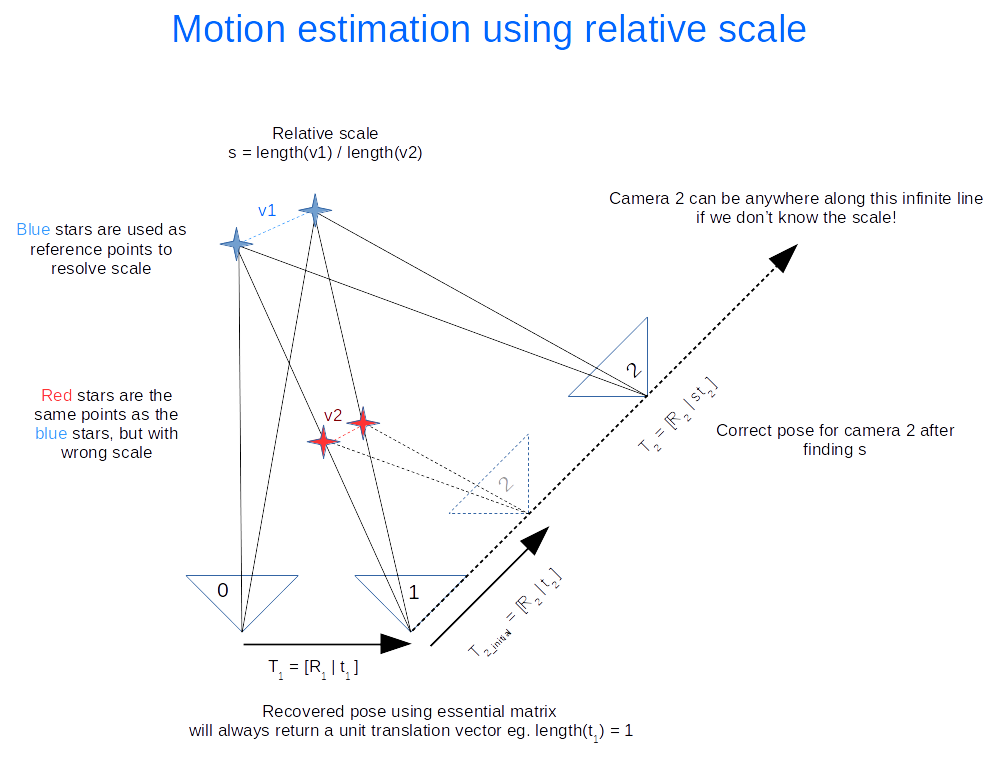
\includegraphics[width=\textwidth]{src/img/nghiaho_2017_sfm_scaling}
    \caption{~\cite{nghiaho_2017}}
    \label{fig:sfm-scaling}
\end{figure}
